\documentclass{standalone}
\usepackage{xcolor,amsmath,amssymb,amsfonts}
\usepackage{fontspec}
\usepackage[T1]{fontenc}
\usepackage[tt=false, type1=true]{libertine}
\usepackage[libertine]{newtxmath}

\usepackage{tikz}
\usetikzlibrary{arrows.meta}
\definecolor{red}{HTML}{c63a44}
\begin{document}

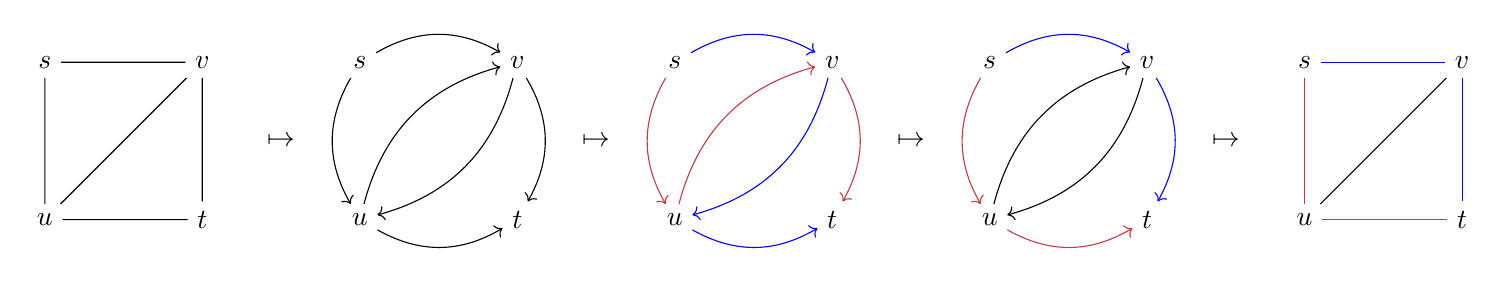
\begin{tikzpicture}
    \node at(0,1)(s1){$s$};
    \node at(0,-1)(u1){$u$};
    \node at(2,1)(v1){$v$};
    \node at(2,-1)(t1){$t$};
    \draw (s1) -- (u1) -- (t1) -- (v1) -- (s1) (v1) -- (u1);
    \node at(3,0){$\mapsto$};
    % 
    \node at(4,1)(s2){$s$};
    \node at(4,-1)(u2){$u$};
    \node at(6,1)(v2){$v$};
    \node at(6,-1)(t2){$t$};
    \draw[->, bend left] (v2) edge (u2) (s2) edge (v2) (v2) edge (t2) (u2) edge (v2);
    \draw[->, bend right] (s2) edge (u2) (u2) edge (t2);
    \node at(7,0){$\mapsto$};
    % 
    \node at(8,1)(s3){$s$};
    \node at(8,-1)(u3){$u$};
    \node at(10,1)(v3){$v$};
    \node at(10,-1)(t3){$t$};
    \draw[->, bend left] (v3) edge[blue] (u3) (s3) edge[blue] (v3) (v3) edge[red] (t3) (u3) edge[red] (v3);
    \draw[->, bend right] (s3) edge[red] (u3) (u3) edge[blue] (t3);
    \node at(11,0){$\mapsto$};
    %
    \node at(12,1)(s4){$s$};
    \node at(12,-1)(u4){$u$};
    \node at(14,1)(v4){$v$};
    \node at(14,-1)(t4){$t$};
    \draw[->, bend left] (v4) edge (u4) (s4) edge[blue] (v4) (v4) edge[blue] (t4) (u4) edge (v4);
    \draw[->, bend right] (s4) edge[red] (u4) (u4) edge[red] (t4);
    \node at(15,0){$\mapsto$};
    % 
    \node at(16,1)(s5){$s$};
    \node at(16,-1)(u5){$u$};
    \node at(18,1)(v5){$v$};
    \node at(18,-1)(t5){$t$};
    \draw (s5) edge[red] (u5) (u5) edge[red](t5) (t5) edge[blue] (v5) (v5) edge[blue](s5) (v5) edge (u5);
\end{tikzpicture}

\end{document}